\documentclass[12pt, a4paper, oneside]{article}

% Extension de capacités
\usepackage{etex}

% Francisation du document
\usepackage[utf8]{inputenc}
\usepackage[T1]{fontenc}
\usepackage[frenchb]{babel}

% Police de caractères
\usepackage{lmodern}
\usepackage{fourier-orns}

% Listes d'énumération
\usepackage{enumitem}

% Mathématiques
\usepackage{mathtools}
\usepackage{mathrsfs}
\usepackage{mathdots}
\usepackage{amssymb}
\usepackage{amsmath}

% Références croisées
\usepackage[french]{varioref}

% Couleurs et boites
\usepackage[x11names]{xcolor}
\usepackage{fancybox}

% Images
\usepackage{graphicx}
\usepackage{wrapfig}

% Subfloat
\usepackage{caption}
\usepackage{subcaption}

\usepackage{eurosym}

% Unités
\usepackage{siunitx}
\sisetup{%
  unitsep = \cdot,%
  decimalsymbol = comma,%
  expproduct = \cdot,%
  seperr,%
  trapambigerr = false,%
  alsoload = hep%
}

% Propriétés hypertexte
\usepackage[pdftex]{hyperref}
\hypersetup{%
  pdfauthor = {Bruneau Basile et Masset Camille, X2013},%
  pdftitle = {INF555 - Rapport de projet},%
  pdfsubject = {},%
  pdfkeywords = {},%
  pdfcreator = {pdfLaTeX},%
  pdfproducer = {pdfLaTeX},%
  bookmarksnumbered = true,%
  pdfstartview = FitH,%
  pdfpagelayout = OneColumn,%
  colorlinks = false,%
  pdfborder = {0 0 0}%
}

\usepackage{listings}

% Package Polytechnique
\usepackage{polytechnique}

% Mes fonctions
% \usepackage[ensemblesGras]{mesfonctions}

\title{INF555 -- Projet}
\subtitle{Sketch-Based Shape Retrieval}
\date{le \today}
\author{Bruneau Basile\\Masset Camille\\\emph{X2013}}


\begin{document}

\renewcommand{\labelitemi}{\starredbullet}
% \setlength{\parskip}{1em}

\maketitle

% \tableofcontents

L'article étudié présente une méthode permettant de retrouver, à partir d'un croquis, un modèle en trois dimensions dans une base de données de \num{1800} objets.

\section{Méthode}

\paragraph{Idée générale.}
La méthode présentée dans l'article repose sur la notion de \emph{bag-of-features}, c'est-à-dire d'ensemble de vecteurs qui caractérisent une image.
La recherche d'un modèle dans une base de données se ramène donc à la recherche d'un vecteur.
Pour mener à bien cette démarche, il faut dans un premier temps générer une bibliothèque de vecteurs associés aux modèles 3D dans laquelle on va effectuer la recherche du vecteur généré à partir du croquis de requête.

\paragraph{Étapes principales de l'algorithme.}
\begin{enumerate}
    \item La première étape consiste donc en la génération de croquis, à partir d'un modèle, tel qu'un humain le ferait.
    \item On découpe les croquis générés en morceaux, et pour chaque morceau, on calcule une \emph{feature}.
    Cela représente donc un ensemble de plusieurs milliers de \emph{features}, qu'on réduit à un millier de représentants par une méthode de classification non supervisée.
    Ces \num{1000} représentants vont constituer notre alphabet.
    \item Enfin on représente chaque croquis par un histogramme correspond au nombre de fois que chaque mot de l'alphabet apparait dans celui-ci.
    Cet histogramme est une sorte de carte d'identité de l'image.
    \item Pour trouver les croquis générés (et donc les modèles) les plus proches d'un dessin, on compare simplement les histogrammes.
    Des histogrammes proches indiquent des dessins proches.
\end{enumerate}


\section{Implémentation}

L'algorithme, que nous avons choisi d'implémenter en \textbf{C++}, se découpe en deux grandes étapes:
\begin{itemize}
    \item un pré-traitement des \num{1800} modèles est d'abord effectué, permettant d'obtenir une nouvelle base de données, composée de l'alphabet de \num{1000} mots et des histogrammes des croquis générés (\emph{offline processing});
    \item la recherche à partir d'un croquis dans cette nouvelle base de données (\emph{online querying}).
\end{itemize}


\subsection{Pré-traitement des modèles}

Lorsqu'une personne réalise un croquis (en deux dimensions) d'un objet, elle effectue plusieurs choix (figure~\vref{img:croquis-exemple}):
\begin{itemize}
    \item elle choisit une direction depuis laquelle regarder, ou selon laquelle projeter l'objet;
    \item elle choisit de quelle façon transformer l'objet texturé qu'elle observe en simple lignes.
\end{itemize}

\begin{figure}
    \begin{center}
        \null\hfill
        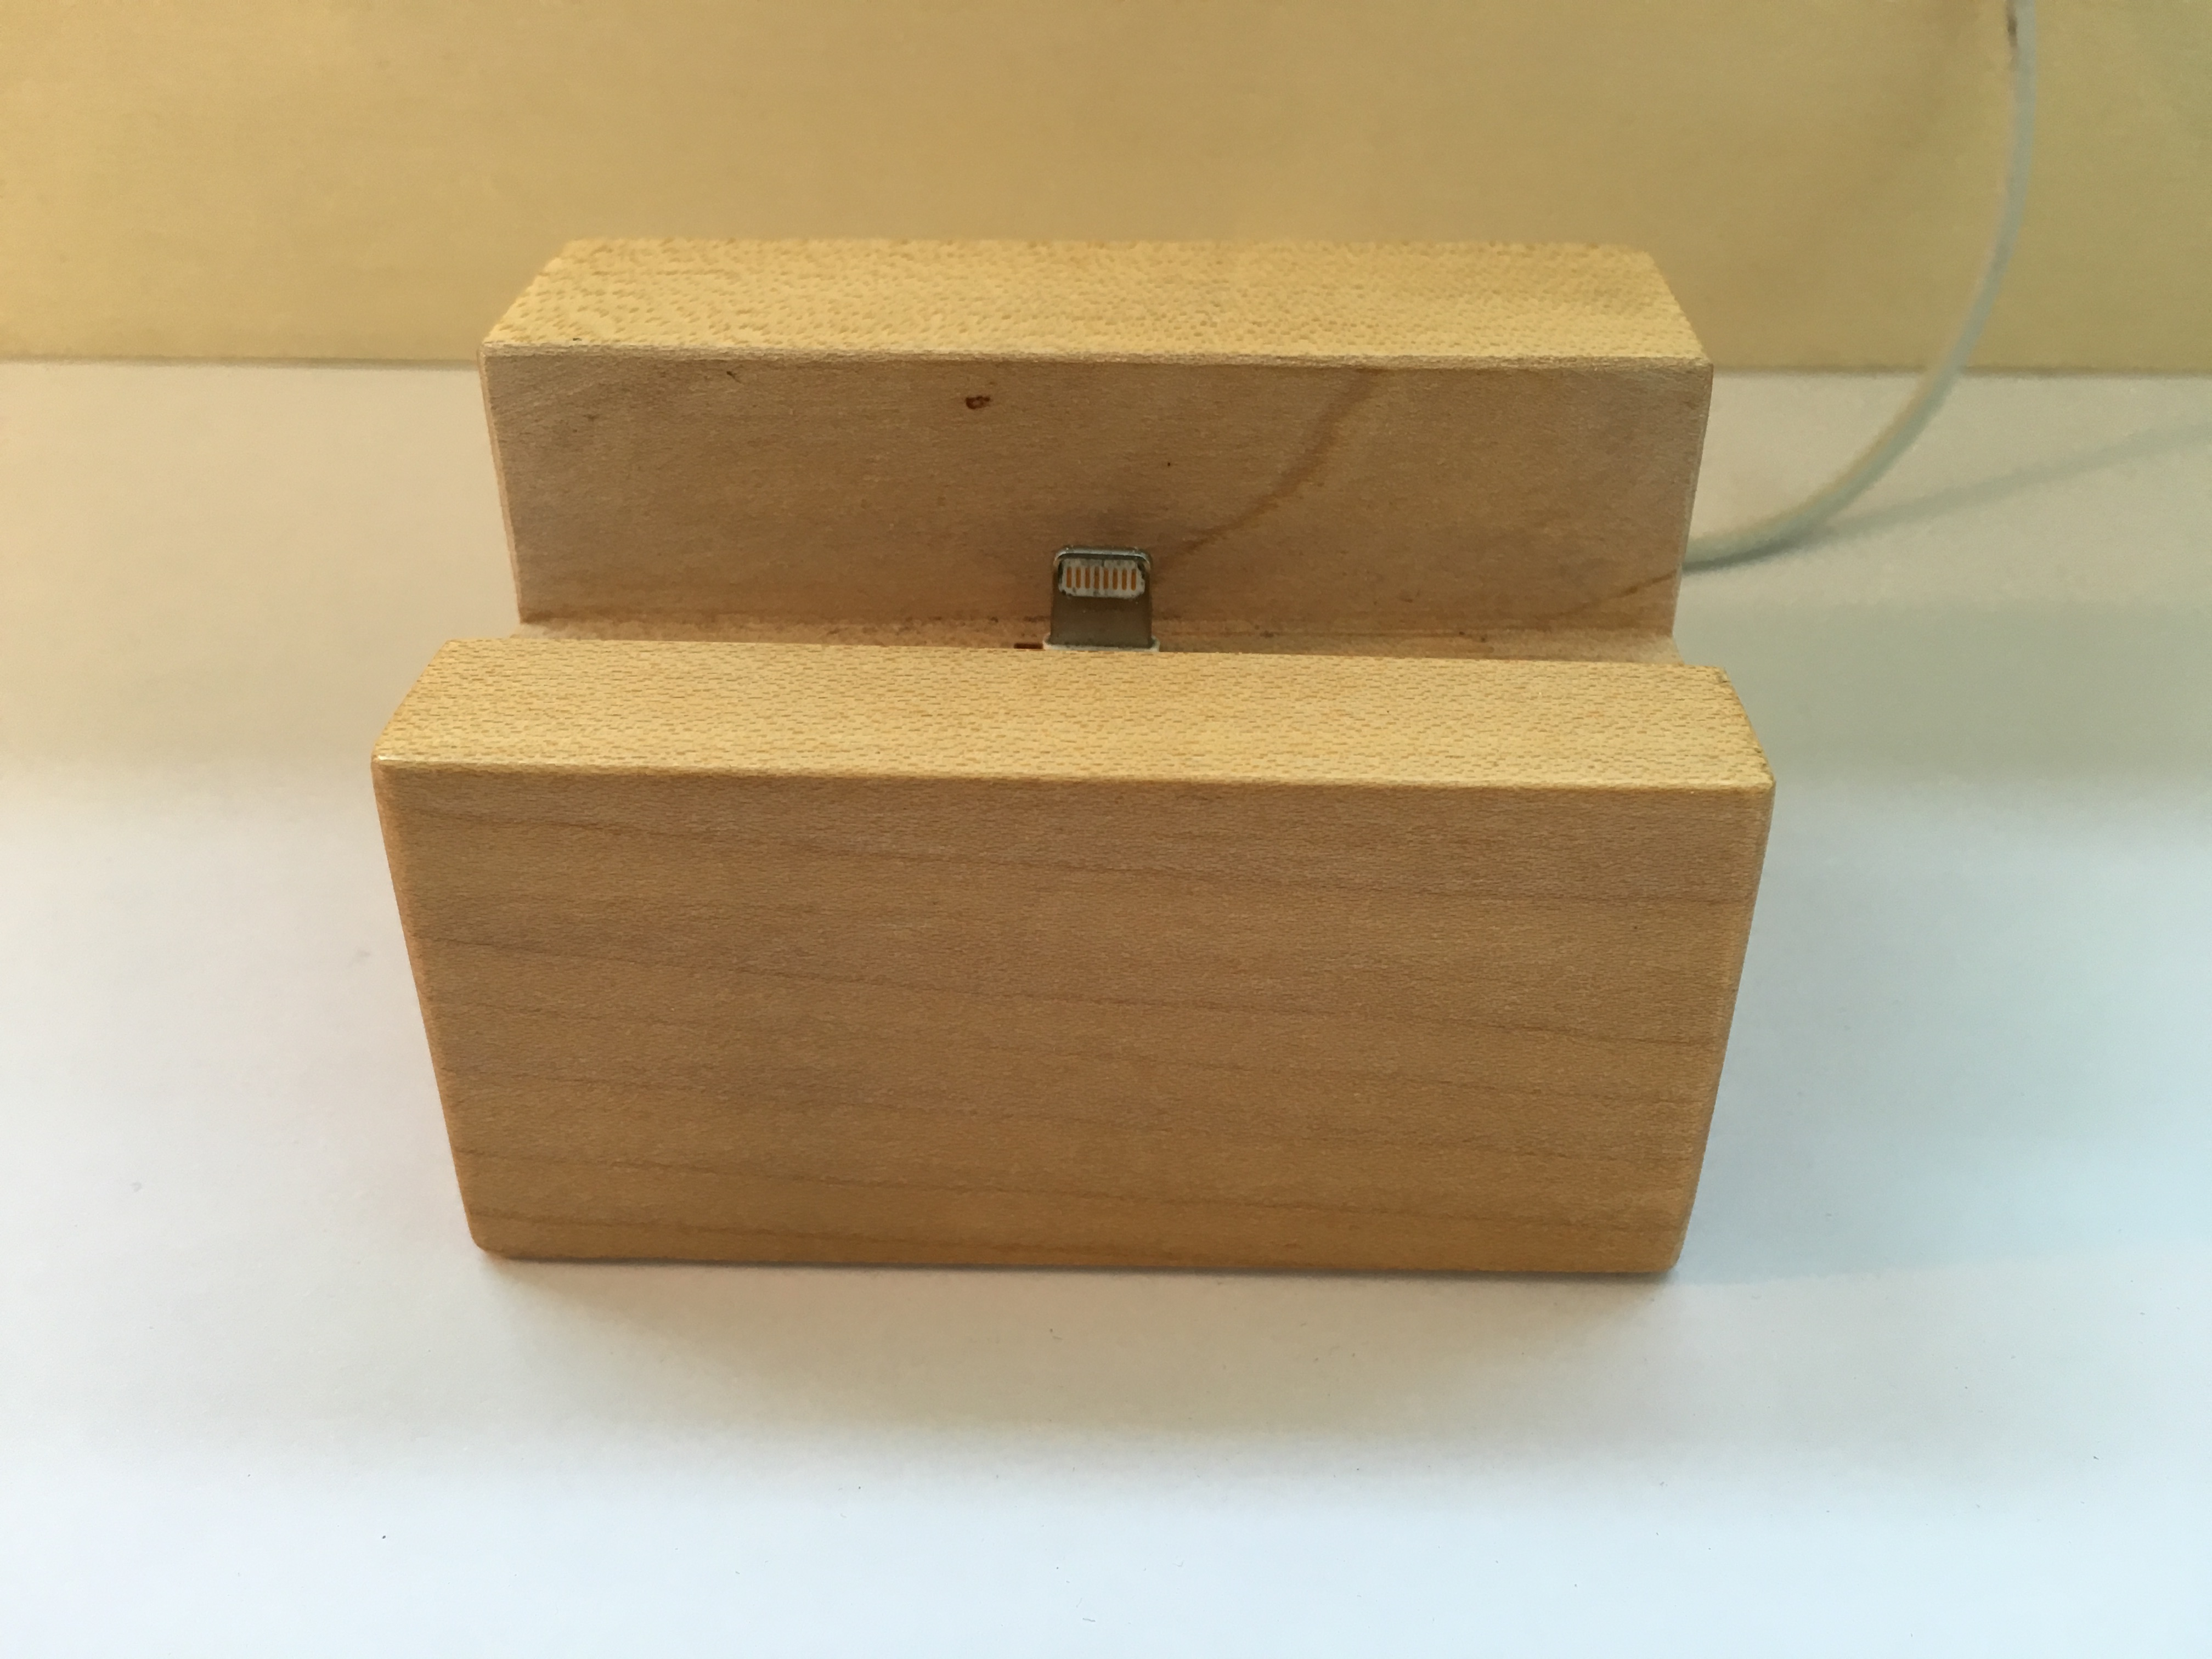
\includegraphics[scale=0.038]{images/dock1.jpg}\hfill
        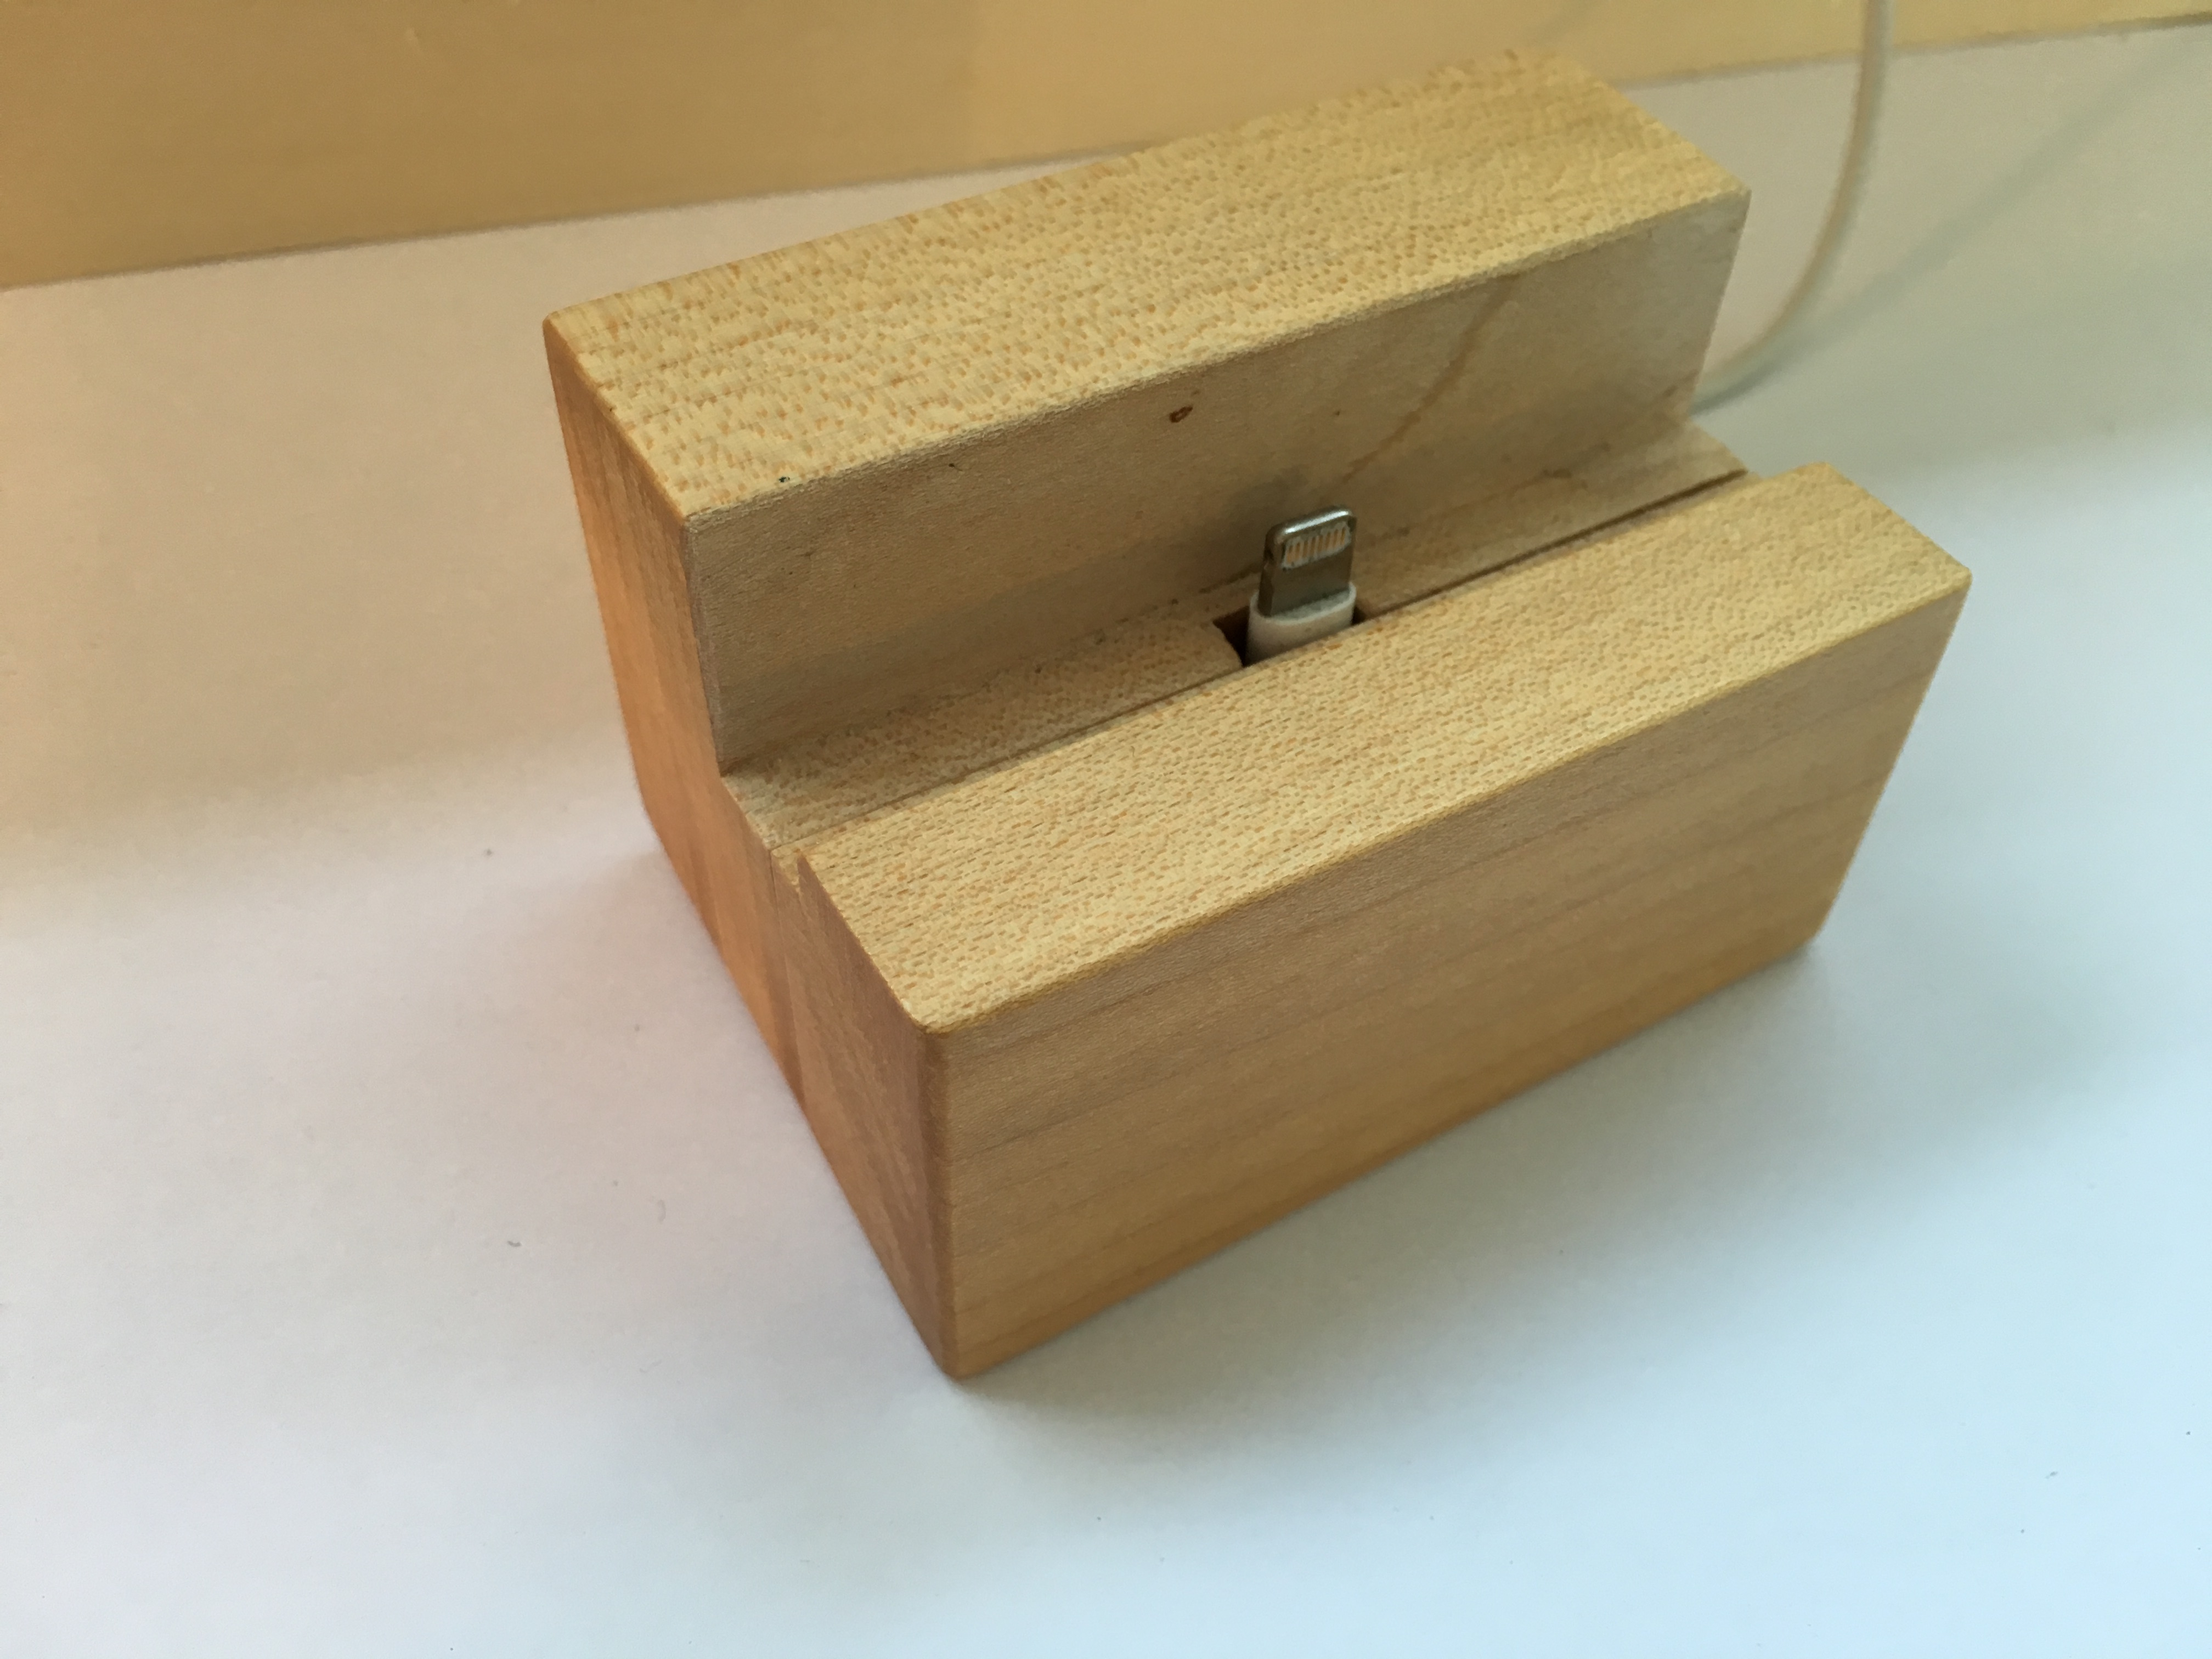
\includegraphics[scale=0.038]{images/dock2.jpg}\hfill
        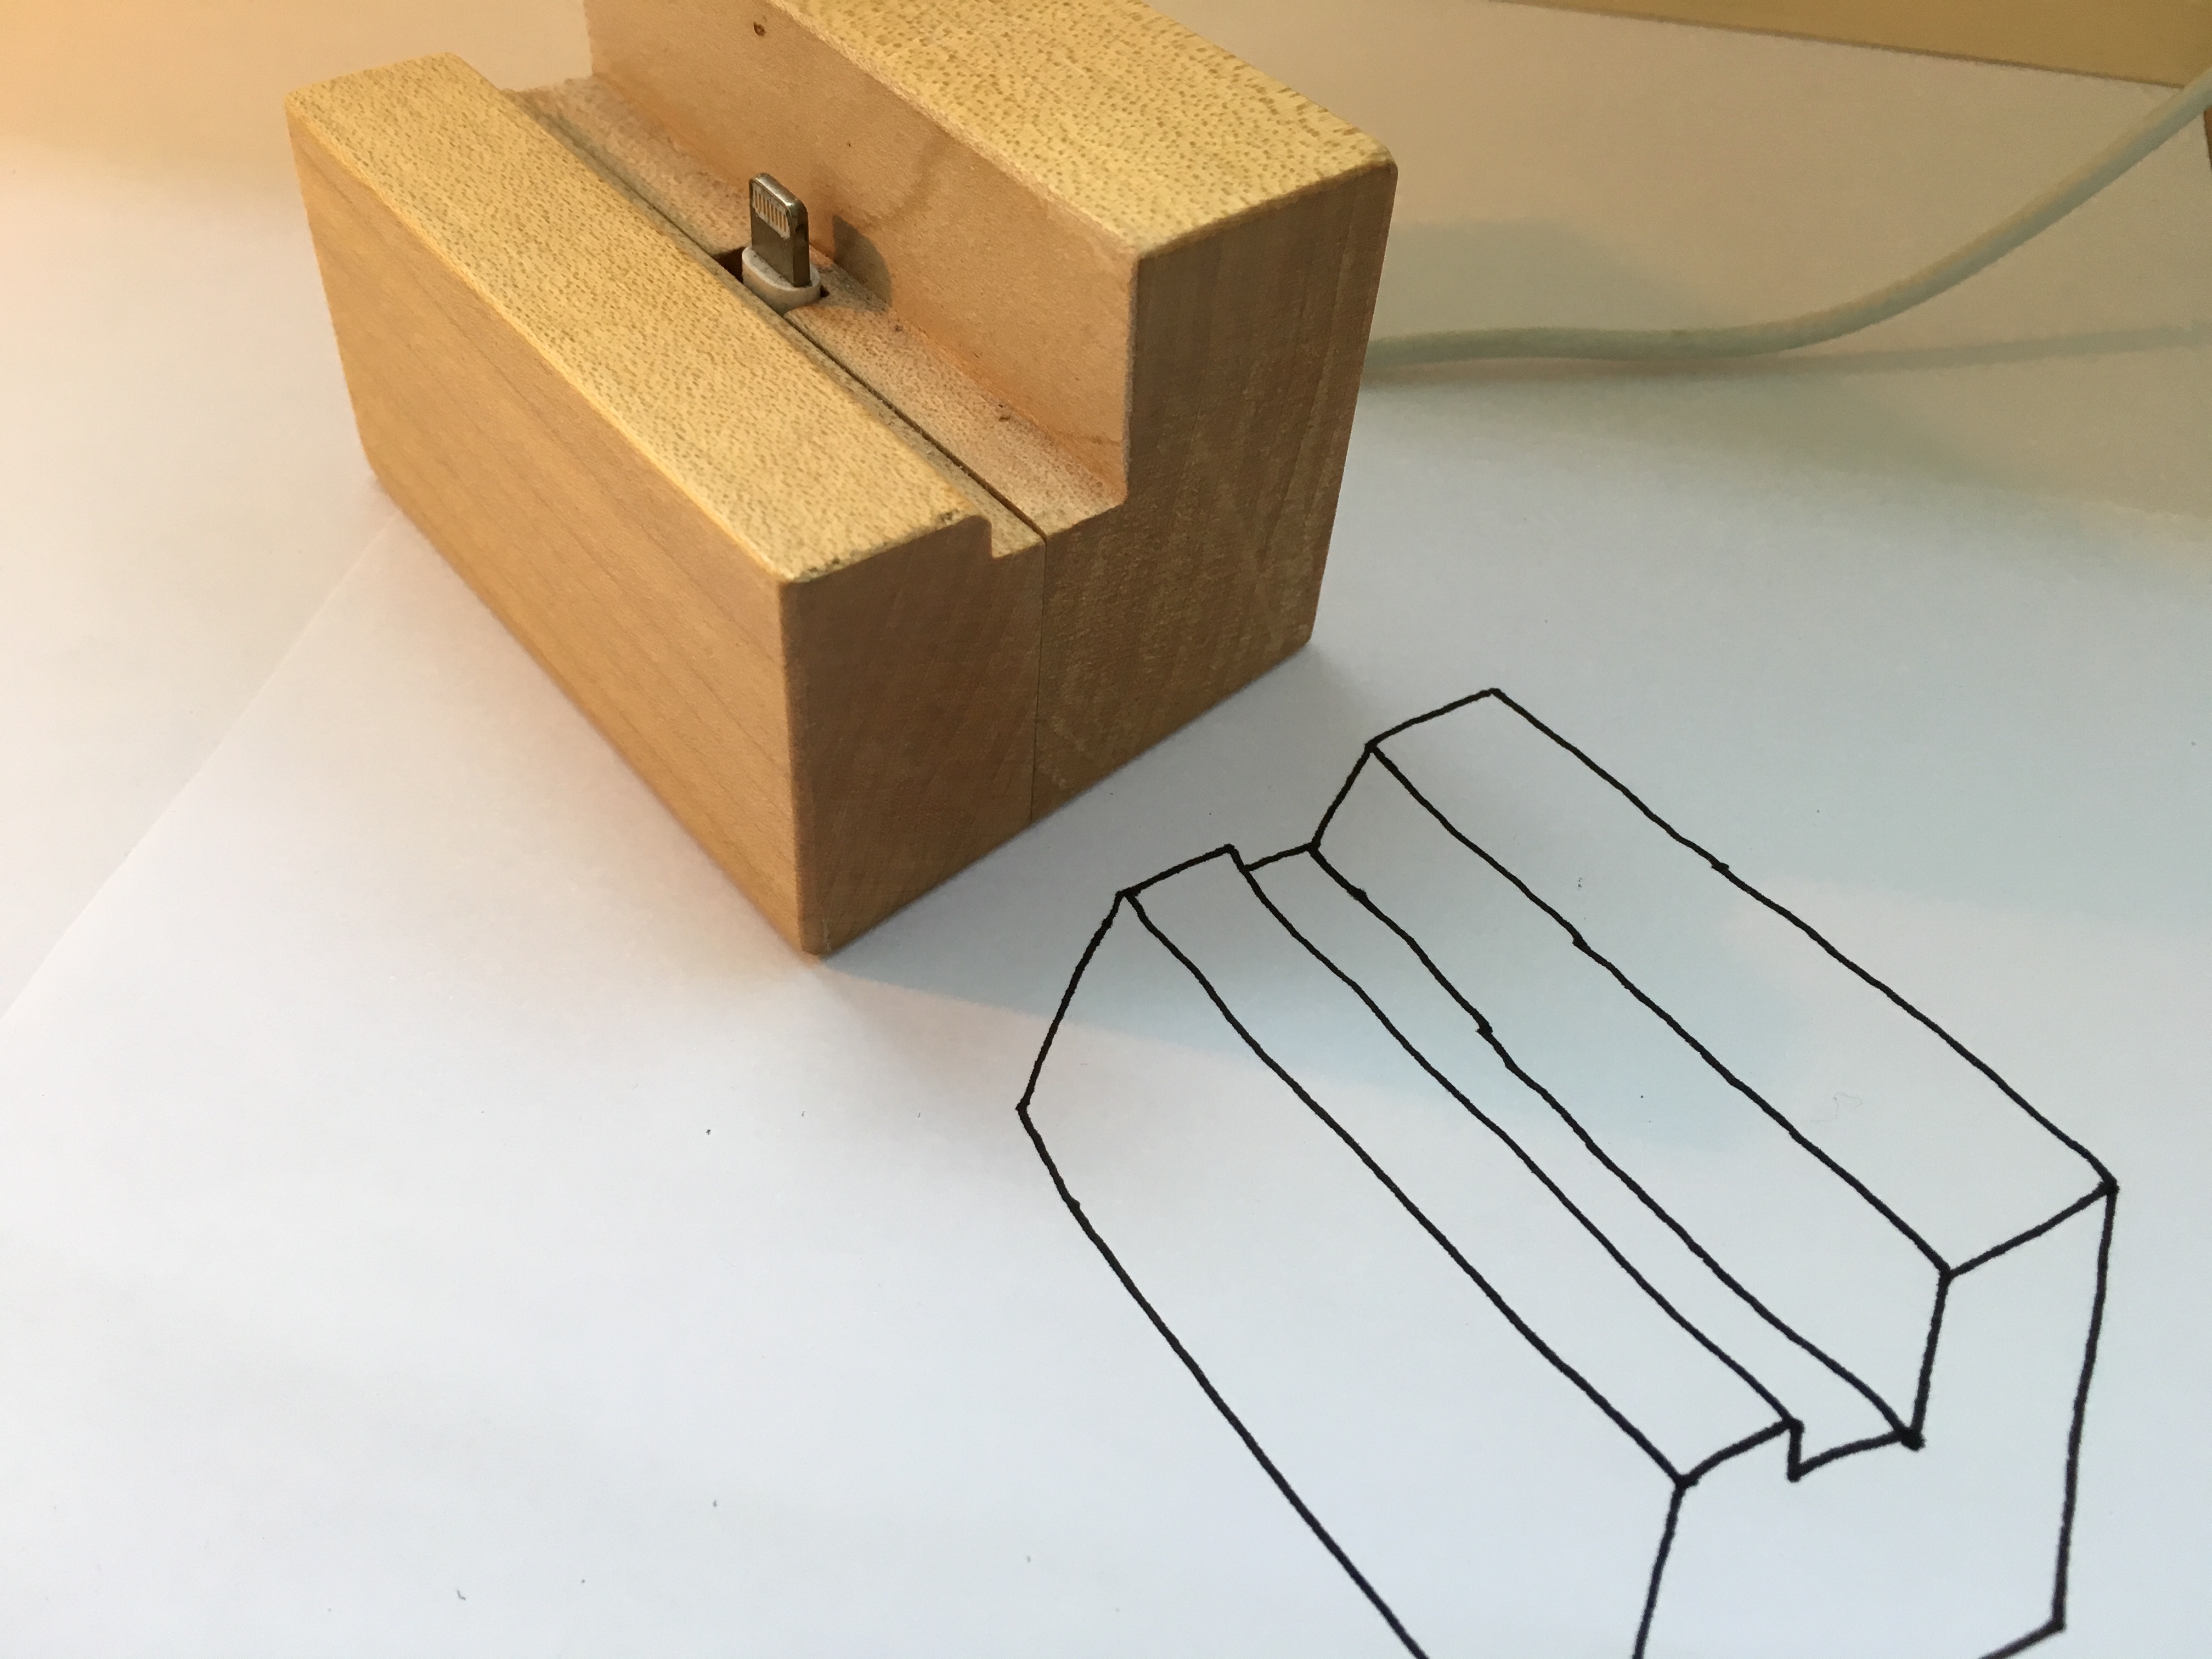
\includegraphics[scale=0.038]{images/dock3.jpg}\hfill\null{}
        \caption{Une orientation a été choisie, et seules certaines lignes sont dessinées.\label{img:croquis-exemple}}
    \end{center}
\end{figure}

Lors de la première étape, pour chaque modèle 3D on génère un ensemble de 50 directions au hasard (mais uniformément réparties) selon lesquelles projeter.
Comme suggéré par l'article on tire 50 points aléatoirement sur une sphère (provenant d'un fichier \verb|.off| composé de \num{16000} sommets) puis on applique l'algorithme \emph{k-means} permettant de séparer la sphère en 50 régions de même taille uniformément réparties.
On prend ensuite le centre de chaque région comme direction de projection.

Pour la deuxième étape, le choix que nous avons fait est de calculer une carte de profondeur de la projection (une image de l'objet où la couleur d'un point dépend de sa distance à l'observateur: un point proche sera noir et un point au loin sera blanc).
On applique ensuite à l'image obtenue un algorithme de détection des contours (Canny).
Nous ouvrons le modèle au format \verb|.off| avec \textbf{OpenGL}, qui nous permet d'obtenir la carte de profondeur. Nous utilisons la bibliothèque \textbf{OpenCV} pour ensuite appliquer le filtre de Canny.

On obtient ainsi un ensemble d'images pour chaque modèle qui ressemblent à des croquis (figure~\vref{img:generer-vues}).

\begin{figure}
    \begin{center}
        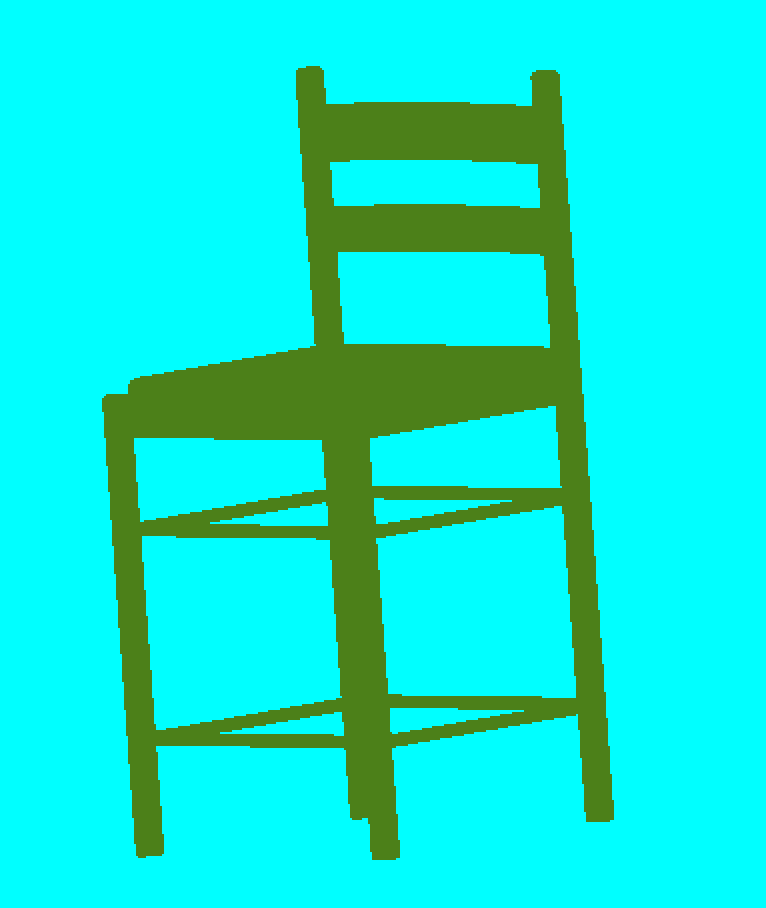
\includegraphics[scale=0.41]{images/chaise-3d.png}
        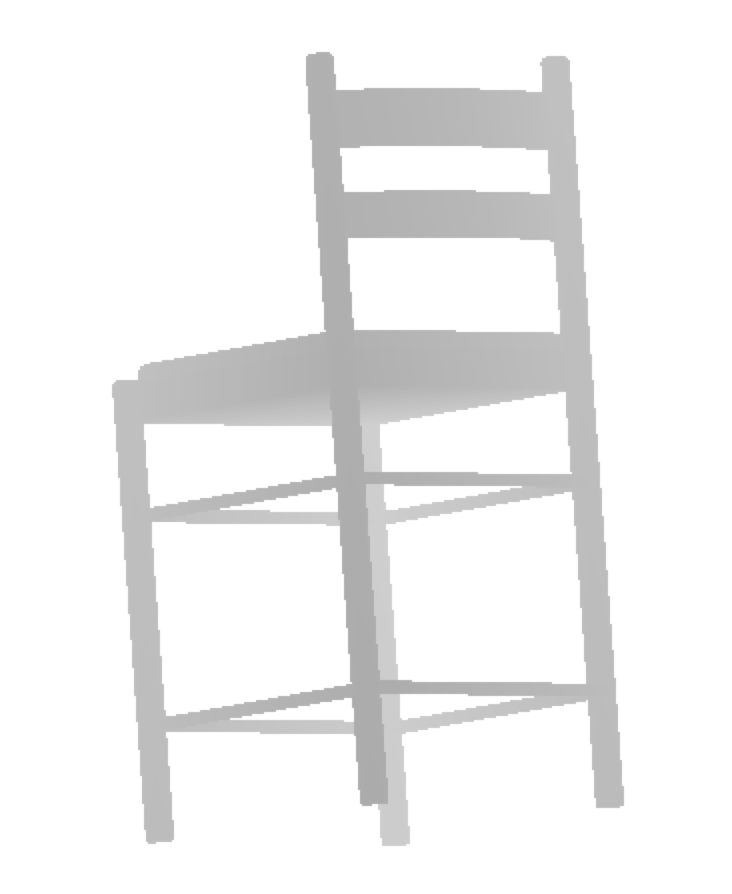
\includegraphics[scale=0.41]{images/chaise-depth.png}
        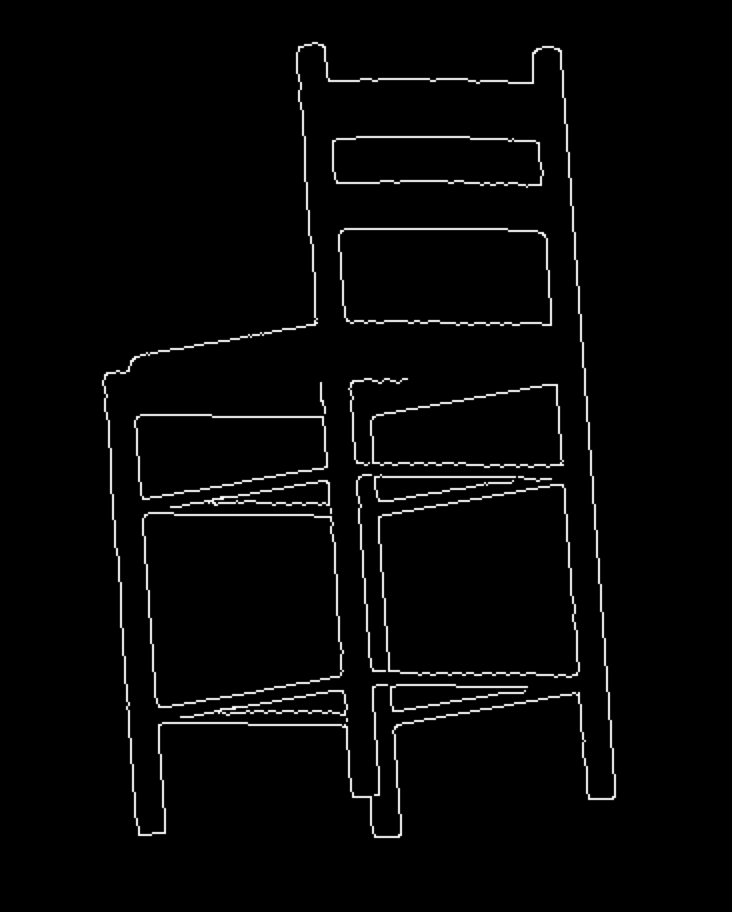
\includegraphics[scale=0.41]{images/chaise-cany.png}
        \caption{Le modèle 3D, la carte de profondeur, puis le résultat après la détection des contours via Canny.\label{img:generer-vues}}
    \end{center}
\end{figure}

Nous effectuons ensuite les étapes suivantes.
\paragraph{Filtre de Gabor.}
Afin d'améliorer les contours, on applique un filtre de Gabor à chaque image, suivant 4 directions.
Cela permet de renforcer les contours dans la direction choisie et d'atténuer les autres.
On calcule pour ça la transformée de Fourier discrète d'une image (avec OpenCV), on la multiplie pixel par pixel au filtre (dans le domaine spectral), puis on revient dans le domaine spatial.
L'article restait assez flou sur les détails techniques de cette partie, qui s'est révélée être chronophage et difficile.
Nous avons en effet rencontré quelques difficultés, en particulier avec la définition du filtre: la formule définissant le filtre dans le domaine spectral était valable pour des fonctions continues mais devait être adaptée pour un usage dans le cas discret.
De plus, la multiplication de matrices complexes implémentées dans OpenCV n'a pas fonctionné.
Ce problème a été particulièrement difficile à détecter mais a pu être résolu.
Enfin, les résultats de filtrage obtenus présentent des artefacts ou effets de bord que nous n'avons pas réussi à éliminer.

\paragraph{Calcul des \emph{features}.}
On découpe les 4 images obtenues en \num{1024} blocs d'aire \SI{7.5}{\percent} de l'aire de l'image.
Chaque bloc est ensuite divisé en 64 cellules.
Pour chaque cellule on somme les valeurs des pixels qu'elle contient.
Ces $64 \times 4 = 256$ valeurs forment un mot (ou \emph{feature}).
Nous stockons ces vecteurs sous forme de tableaux de flottants.
Nous avons pu constater la difficulté de gérer correctement la mémoire en \textbf{C++}, notamment quand on emploie des \emph{pointeurs}.
Finalement, au lieu de stocker les vecteurs avec des \verb|float*|, nous avons utilisé le conteneur fourni par la librairie standard \verb|std::array<float, FEAT_SIZE>|, ce qui nous a permis de nous affranchir de l'usage des pointeurs.

\paragraph{Constitution d'un vocabulaire visuel.}
On élimine aléatoirement une partie de ces mots afin de n'en garder qu'un million.
Cela représente néanmoins un volume d'environ \num{256}~Mo.
Grâce à l'algorithme \emph{k-means}, on réduit ce million de mots à un millier, qui vont composer notre alphabet.

\paragraph{Indexation des modèles.}
Enfin on calcule l'histogramme de chaque image en regardant pour chacun de ses \num{1024} mots de quel mot de l'alphabet il est le plus proche, au sens de la métrique euclidienne.


Cet ensemble d'étapes pouvant s'avérer très long (une vingtaine d'heures pour les \num{1800} modèles), nous stockons le résultat obtenu (l'alphabet et les histogrammes) dans un fichier.
De façon générale, l'article passait sous silence toute question relative à l'efficacité, mais c'est un problème auquel nous avons dû être très attentifs.
En effet, avec \num{1800} modèles, 50 projections par modèles et \num{1024} mots de longueur 256 par projection, on peut facilement atteindre 20~Go en mémoire.


\subsection{Recherche d'un modèle}

On commence par charger en mémoire l'alphabet et les histogrammes des modèles à partir du fichier dans lequel nous avions sauvegardé ces données.

Lorsqu'on donne un croquis au programme, on calcule son histogramme comme précédemment (on applique Canny, on filtre par Gabor suivant différentes orientations et on déceoupe en blocs pour calculer les \emph{features}).
Ensuite on cherche simplement de quels histogrammes il est le plus proche.


\section{Résultats}

\subsection{Pré-traitement}

\paragraph{Filtre de Gabor/}
On a commencé par vérifier que le filtre de Gabor donnait des résultats attendus, à savoir, intensifier les contours dans une certaine direction.
Sur la figure~\vref{fig:result-gabor}, on peut constater que pour $\theta = \pi/4$, ce résultat est obtenu, malgré quelques effets de bords.
\begin{figure}
    \begin{center}
        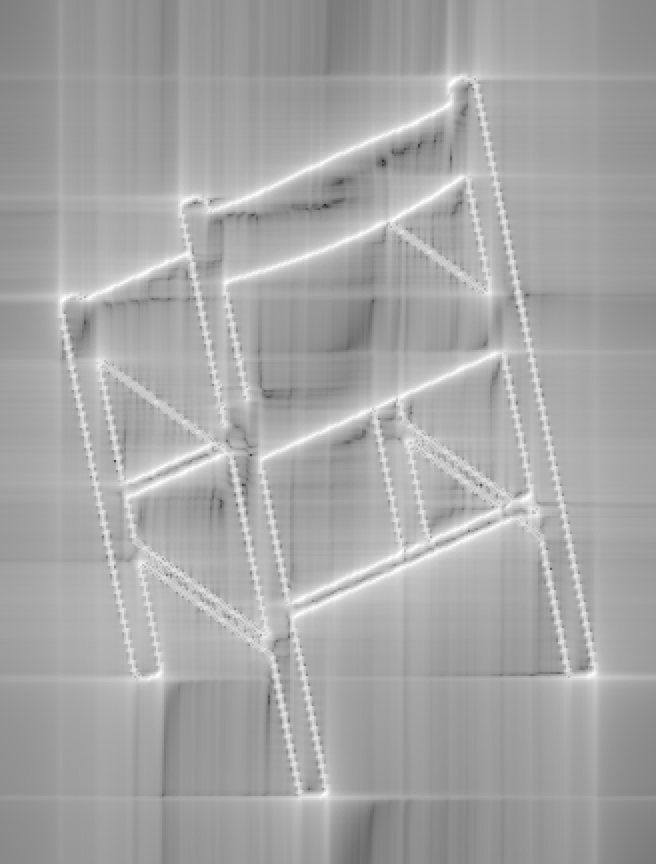
\includegraphics[width=0.4\textwidth]{images/chair-gabor}
        \caption{Filtrage d'une chaise par Gabor.\label{fig:result-gabor}}
    \end{center}
\end{figure}

\paragraph{Chaine de traitement complète/}
Pour constituer notree vocabulaire visuel et notre base de données d'histogrammes, on a choisi les paramètres suivants:
\begin{itemize}
    \item nombre de modèles 3D: 100 (chaises, voitures, avions, \ldots);
    \item nombre de vues par modèle: 50;
    \item taille du vocabulaire: 50 mots\footnote{on a ainsi le même rapport nombre total de vues sur taille du vocabulaire que les auteurs, à savoir 100.}.
\end{itemize}
Le temps d'exécution a été d'environ 50 minutes. Il est à noter que la mémoire utilisée n'a pas excédée 150 MB.

On obtient alors un fichier contenant:
\begin{itemize}
    \item la longueur des mots, le nombres de mots (taille du vocabulaire) et le nombre de total de vues sur la première ligne;
    \item une ligne par mot: la fréquence de ce mot dans le vocabulaire, suivie des 256 coordonnées du mot;
    \item une ligne par vue: le nom du modèle associé, suivi des valeurs de l'histogramme.
\end{itemize}
Ce fichier pèse quelques MB.


\subsection{Requêtes}
L'étape de \emph{querying} est beaucoup plus rapide.
Après l'importation des données du fichier d'histogrammes, qui s'effectue quasiment instantanément, on calcule simplement un histogramme.
Ensuite, on cherche les histogrammes les plus proches dans la base de données.
On peut choisir le nombre de résultats souhaités.
La figure~\vref{fig:query-result} montre les résultats obtenus pour un croquis donné en entrée.
\begin{figure}
    \begin{center}
        \includegraphics[width=.3\textwidth]{images/query-sketch}\hfill
        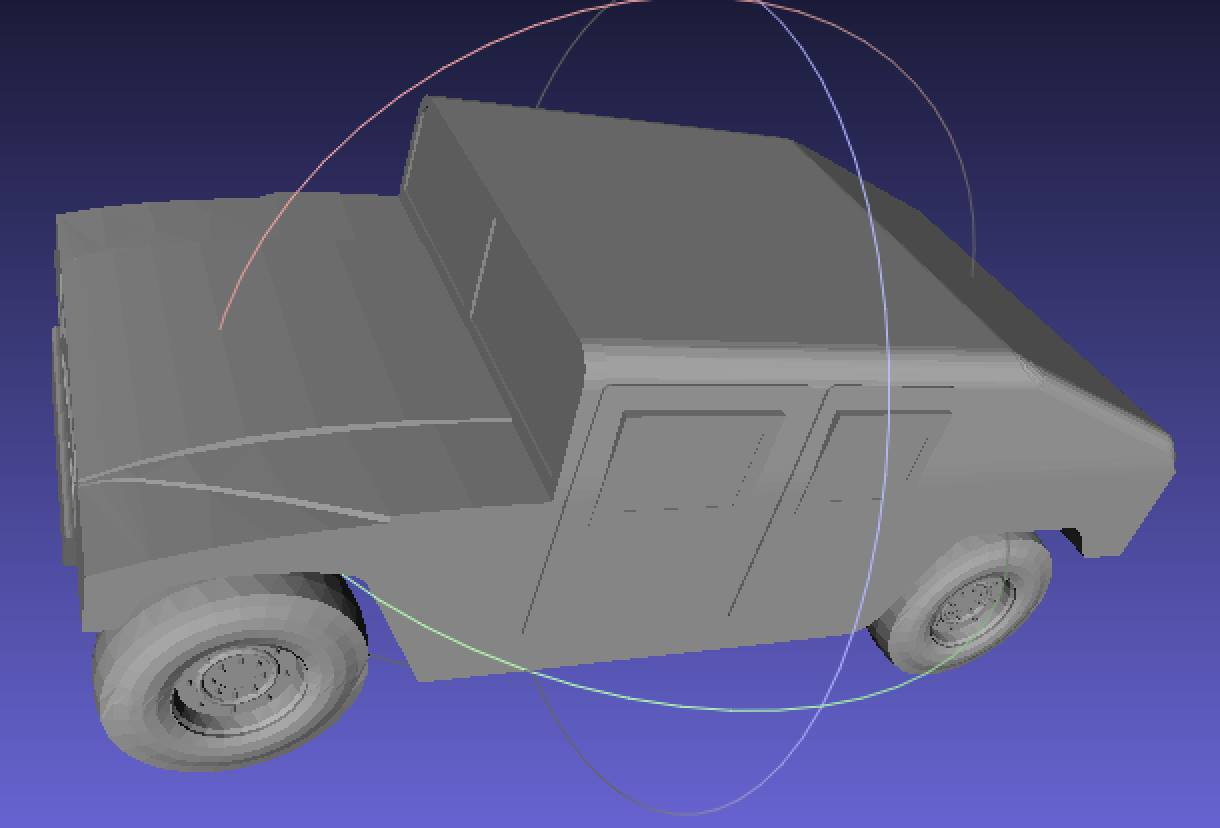
\includegraphics[width=.3\textwidth]{images/query-result1}
        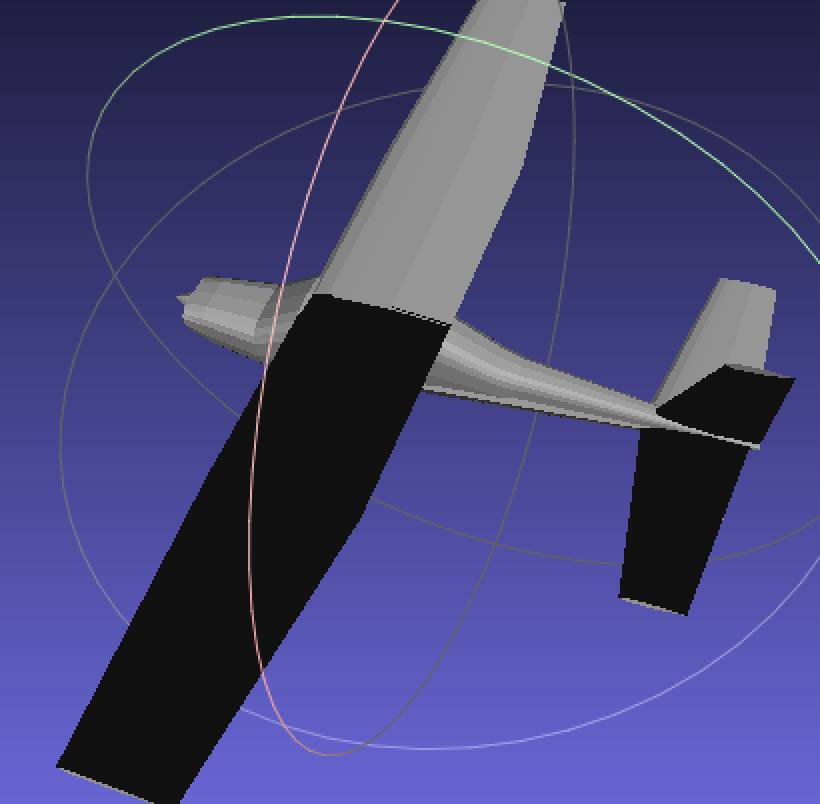
\includegraphics[width=.3\textwidth]{images/query-result2}
    \end{center}
\end{figure}


\section{Pistes d'amélioration}

Tout au long du projet, nous avons fait des choix, car l'article proposait souvent plusieurs solutions.

Nous choisissons les directions selon lesquelles projeter le modèle de manière aléatoire mais uniforme.
Une autre possibilité est d'essayer de calculer la probabilité d'une projection en utilisant plusieurs facteurs tels que la longueur de la projection, l'aire de la projection, et les variations de profondeur.

Pour l'obtention des croquis à partir des modèles 3D, nous avons décidé d'appliquer Canny à la carte de profondeur.
Cela donne de bons résultats, mais l'algorithme \emph{Suggestive Contours} qui s'applique directement au modèle 3D pourrait donner de meilleurs résultats.

Nous pourrions également augmenter la résolution des projections, qui est actuellement limitée à $800 \times 800$.
Généralement les contours sont assez fins (4 à 5~pixels) et peu lisses.

Il est également possible d'agir sur le nombre de projections réalisées pour chaque modèle.
Nous nous sommes limités à 50 pour des raisons d'efficacité, mais les auteurs suggèrent 100.


\end{document}
